\documentclass[a4paper]{article}
\usepackage{a4wide,amssymb,epsfig,latexsym,multicol,array,hhline,fancyhdr}
\usepackage{vntex}
\usepackage{amsmath}
\usepackage{lastpage}
\usepackage[lined,boxed,commentsnumbered]{algorithm2e}
\usepackage{enumerate}
\usepackage{color}
\usepackage{graphicx}							
% Standard graphics package
\usepackage{xcolor}
\usepackage{listings}
\colorlet{mygray}{black!30}
\colorlet{mygreen}{green!60!blue}
\colorlet{mymauve}{red!60!blue}

\lstset{
  backgroundcolor=\color{gray!10},  
  basicstyle=\ttfamily,
  columns=fullflexible,
  breakatwhitespace=false,      
  breaklines=true,                
  captionpos=b,                    
  commentstyle=\color{mygreen}, 
  extendedchars=true,              
  frame=single,                   
  keepspaces=true,             
  keywordstyle=\color{blue},      
  language=R,                 
  numbers=none,                
  numbersep=5pt,                   
  numberstyle=\tiny\color{blue}, 
  rulecolor=\color{mygray},        
  showspaces=false,               
  showtabs=false,                 
  stepnumber=5,                  
  stringstyle=\color{mymauve},    
  tabsize=3,                      
  title=\lstname                
}
\usepackage{extarrows}

\usepackage{array}
\usepackage{tabularx, caption}
\usepackage{multirow}
\usepackage{multicol}
\usepackage{rotating}
\usepackage{graphics}
\usepackage{geometry}
\usepackage{setspace}
\usepackage{epsfig}
\usepackage{tikz}
\usetikzlibrary{arrows,snakes,backgrounds}
\usepackage{hyperref}
\hypersetup{urlcolor=blue,linkcolor=black,citecolor=black,colorlinks=true} 
%\usepackage{pstcol} 								% PSTricks with the standard color package


\newtheorem{theorem}{{\bf Theorem}}
\newtheorem{property}{{\bf Property}}
\newtheorem{proposition}{{\bf Proposition}}
\newtheorem{corollary}[proposition]{{\bf Corollary}}
\newtheorem{lemma}[proposition]{{\bf Lemma}}

\AtBeginDocument{\renewcommand*\contentsname{Contents}}
\AtBeginDocument{\renewcommand*\refname{References}}
%\usepackage{fancyhdr}
\setlength{\headheight}{40pt}
\pagestyle{fancy}
\fancyhead{} % clear all header fields
\fancyhead[L]{
 \begin{tabular}{rl}
    \begin{picture}(25,15)(0,0)
    \put(0,-8){
\includegraphics[width=8mm, height=8mm]{hcmut.png}}
    %\put(0,-8){\epsfig{width=10mm,figure=hcmut.eps}}
   \end{picture}&
	%
\includegraphics[width=8mm, height=8mm]{hcmut.png} & %
	\begin{tabular}{l}
		\textbf{\bf \ttfamily University of Technology, Ho Chi Minh City}\\
		\textbf{\bf \ttfamily Faculty of Computer Science and Engineering}
	\end{tabular} 	
 \end{tabular}
}
\fancyhead[R]{
	\begin{tabular}{l}
		\tiny \bf \\
		\tiny \bf 
	\end{tabular}  }
\fancyfoot{} % clear all footer fields
\fancyfoot[L]{\scriptsize \ttfamily Assignment for Mathematical Modeling -  Academic year 2021 - 2022}
\fancyfoot[R]{\scriptsize \ttfamily Page {\thepage}/\pageref{LastPage}}
\renewcommand{\headrulewidth}{0.3pt}
\renewcommand{\footrulewidth}{0.3pt}


%%%
\setcounter{secnumdepth}{4}
\setcounter{tocdepth}{3}
\makeatletter
\newcounter {subsubsubsection}[subsubsection]
\renewcommand\thesubsubsubsection{\thesubsubsection .\@alph\c@subsubsubsection}
\newcommand\subsubsubsection{\@startsection{subsubsubsection}{4}{\z@}%
                                     {-3.25ex\@plus -1ex \@minus -.2ex}%
                                     {1.5ex \@plus .2ex}%
                                     {\normalfont\normalsize\bfseries}}
\newcommand*\l@subsubsubsection{\@dottedtocline{3}{10.0em}{4.1em}}
\newcommand*{\subsubsubsectionmark}[1]{}
\makeatother


\begin{document}

\begin{titlepage}
\begin{center}
VIETNAM NATIONAL UNIVERSITY, HO CHI MINH CITY \\
UNIVERSITY OF TECHNOLOGY \\
FACULTY OF COMPUTER SCIENCE AND ENGINEERING
\end{center}

\vspace{1cm}

\begin{figure}[h!]
\begin{center}

\includegraphics[width=3cm]{hcmut.png}
\end{center}
\end{figure}

\vspace{1cm}


\begin{center}
\begin{tabular}{c}
\multicolumn{1}{l}{\textbf{{\Large MATHEMATICAL MODELING (CO2011)}}}\\
~~\\
\hline
\\
\multicolumn{1}{l}{\textbf{{\Large Assignment}}}\\
\\
\textbf{{\Huge Process Mining}}\\
\\
\textbf{{\Huge PETRI NETWORKS}}\\
\\
\hline
\end{tabular}
\end{center}

\vspace{1 cm}

\begin{center}
\begin{table}[h]
\begin{tabular}{rrl}
\hspace{2 cm} & Advisor: & Nguyễn Tiến Thịnh.\\
& Team name: &Team Aesthetic. \\
& Students: & Phạm Huy Thanh - 1952977 - CC02 (Leader). \\
& & Vũ Tiến Giang - 1952240 - CC02. \\
& & Nguyễn Trọng Nghĩa - 1951175 - CC01. \\
& & Phan Quang Thiện - 1952997 - CC02. \\
& & Phạm Bá Trọng - 1953045 - CC06. \\
& & Đoàn Việt Tú - 1952521 - CC02. \\
\end{tabular}
\end{table}
\end{center}

\vspace{1 cm}

\begin{center}
{\footnotesize HO CHI MINH CITY, NOVEMBER 2021}
\end{center}
\end{titlepage}


%\thispagestyle{empty}

\newpage
\tableofcontents
\newpage


%%%%%%%%%%%%%%%%%%%%%%%%%%%%%%%%%%%%%%%%%%%%%%%%%%%%%%%%%%%%%%%%%%%%%%%%%%%%%%%%%%%%%%%%%%%%%%%%%%%
\section{Member list \& Workload}

\begin{center}
\begin{tabular}{|c|c|c|l|c|}
\hline
\textbf{No.} & \textbf{Fullname} & \textbf{Student ID} & \textbf{Problems} & \textbf{Percentage}\\
 & & & & \textbf{of work}\\
\hline 
%%%%%Student 1%%%%%%%%%%
\multirow{3}{*}{1} & \multirow{3}{*}{Phạm Huy Thanh} & \multirow{3}{*}{1952977} & - Prepare theory & 
\multirow{3}{*}{16\%}\\
 & &  & - Write Latex: part 3, 4, 5 &\\
 & &  & &\\
\hline 
%%%%%Student 2%%%%%%%%%%%
\multirow{3}{*}{2} & \multirow{3}{*}{Vũ Tiến Giang} & \multirow{3}{*}{1952240} & - Prepare theory & 
\multirow{3}{*}{17\%}\\
 & &  & - Write Latex: part 2, 5, 6 &\\
 & &  & &\\
\hline
%%%%%Student 3%%%%%%%%%%%
\multirow{3}{*}{3} & \multirow{3}{*}{Nguyễn Trọng Nghĩa} & \multirow{3}{*}{1951175} & - Assignment part 6 & 
\multirow{3}{*}{17\%}\\
 & &  & (Supported by Giang and Thanh) &\\
 & &  & &\\
\hline
%%%%%Student 4%%%%%%%%%%%
\multirow{3}{*}{4} & \multirow{3}{*}{Phan Quang Thiện} & \multirow{3}{*}{1952997} &  & 
\multirow{3}{*}{16\%}\\
 & &  & - Exercises and examples &\\
 & &  & &\\
\hline
%%%%%Student 5%%%%%%%%%%%
\multirow{3}{*}{5} & \multirow{3}{*}{Phạm Bá Trọng} & \multirow{3}{*}{1953045} & & \multirow{3}{*}{17\%}\\
 & &  & - Summary part 5 &\\
 & &  & &\\
\hline
%%%%%Student 6%%%%%%%%%%%
\multirow{3}{*}{6} & \multirow{3}{*}{Đoàn Việt Tú} & 
\multirow{3}{*}{1952521} & - Exercise and problems codes & \multirow{3}{*}{17\%}\\
 & &  & - Review the report &\\
 & &  & (Supported by Thiện and Trọng) &\\
\hline
\end{tabular}
\end{center}

%%%%%%%%%%%%%%%%%%%%%%%%%%%%%%%%%%%%%%%%%%%%%%%%%%%%%%%%%%%%%%%%%%%%%%%%%%%%%%%%%%%%%%%%%%%%%%%%%%%
\vspace{1 cm}

\section{PETRI NETWORKS- Background}
\subsection{The Art of Modeling- motivated from Operation Research}
\subsubsection{Definition of Operation Research}
\textbf{Operations Research} (OpRe) is a branch of management science heavily relying on modeling, also called Decision Science or Operations Analysis, is the study of applying mathematics to business questions. As a sub-field of Applied Mathematics, it has a very interesting position alongside other fields as Data Science and Machine Learning.
\subsubsection{Some examples of OpRe:}
\begin{itemize}
    \item Linear Programming
    \item Waiting line theory or queuing theory
    \item Inventory control systems
    \item Replacement problems
    \item Network Analysis
    \item Sequencing Problems
\end{itemize}
\subsection{Petri net}
A \textbf{Petri net}, also known as a place/transition (PT) net, is one of several mathematical modeling languages for the description of distributed systems. It is a class of discrete event dynamic system.\newline
We can define it is a directed bipartite graph that has two types of elements, places and transitions, depicted as white circles and rectangles, respectively. A place can contain any number of tokens, depicted as black circles. A transition is enabled if all places connected to it as inputs contain at least one token.\newline
Some sources state that \textbf{Petri nets} were invented in August 1939 by Carl Adam Petri — at the age of 13 — for the purpose of describing chemical processes.
\subsection{Formal definitions}
\textbf{Petri nets} are state-transition systems that extend a class of nets called elementary nets.
\subsubsection{Definition 1 (Transition system or State transition system)}
Formally, a \textbf{transition system} is a pair $(S, \rightarrow)$, where 
\begin{itemize}
    \item $S$ is a set of states.
    \item $\rightarrow$ is a relation of state transitions (a subset of $S \times S$).
\end{itemize}
A \textbf{labelled transition system} is a tuple $(S, \Lambda, \rightarrow)$, where 
\begin{itemize}
    \item $S$ is a set of states.
    \item $\Lambda$ is a set of labels.
    \item $\rightarrow$ is a relation of labelled transitions $(S, \Lambda, S$).
\end{itemize}
It also can be present as $TS = (S, A, T)$, where 
\begin{itemize}
    \item $S$ is a set of states.
    \item $A \subseteq \Lambda$ is set of activities (also called actions).
    \item $T \subseteq (S \times A \times S)$.
\end{itemize}
The following subsets are defined implicitly,
\begin{itemize}
    \item $S^{start} \subseteq S$ is the set of initial states (sometimes referred to as ‘start’ states).\newline
    $S^{end} \subseteq S$ is the set of final states (sometimes referred to as ‘accept’ states).\newline
    For most practical applications the state space $S$ is finite.
    \item Activities can be executed sequentially, activities can be optional or concurrent, and the repeated execution of the same activity may be possible. Using transition systems in a process model will help arrange the \textit{order} of activities and determine \textit{which activities} need to be executed.
    \item The net structure and dynamic of a transition system may be used to study and express its \textit{behavior}. One of the first states is where the transition begins. A conceivable \textit{execution sequence} corresponds to any path in the graph that starts in this state.
\end{itemize}
A transition system of a vending machine:
\begin{center}
    \includegraphics[width=10cm]{Picture21.png}
\end{center}

\begin{center}
    \includegraphics[width=14cm]{Picture13.png}\\
\end{center}

\vspace{1 cm}

\textbf{Example 5.1.} \text{Observe a transition system in Figure 5.2}
\par
$A = \{register request , examine thoroughly , examine casually , check ticket ,$\par
$reinitiate request , decide , reject request , pay compensation\}$
\par\null\par
$T =\{(s1,register request , s2) ,(s2 , examine casually , s3),(s2, check ticket ,s4),$\par
$(s2,examine thoroughly ,s3),(s3,check ticket,s5),(s4 , examine casually,s5),$\par
$(s4,examine thoroughly ,s5),(s5,decide,s6),(s6, reinitiate request ,s2),$\par
$(s6,reject request,s7),(s6, pay compensation, s7)\}$

\vspace{1 cm}

\textbf{Example 5.2.} \text{A multi-set example}
\par
$M = [a,b,b,c,c,c,d,d,e] = \{a,b^2,c^3,d^2,e\}  = \{e,c^3,b^2,e,d^2\} = [1,3,2,1,2]$

\subsubsection{Definition 2 (Petri Net is a bipartite directed graph N of places and transitions)}
A Petri net is a triplet $N = (P, T, F)$ where
\begin{itemize}
    \item $P$ is a finite set of places.
    \item $T$ is also a finite set of transitions, which P and T are disjoint.
    \item $F \subseteq (P \times T) \cup (T \times P)$ is a set of (directed) arcs, called the flow relation.
\end{itemize}
Remarks:
\begin{itemize}
    \item If the diagram were of an elementary net, then those places in a configuration would be conventionally depicted as circles, where each circle encompasses a single dot called a \textit{token}. It is a special \textit{transition node}, being graphically rendered as a black dot. \textbf{Note:} \textit{Places} can contain tokens but the \textit{transitions} \textbf{cannot}.
    \item A transition is \textit{enabled} if each of its input places contains a token.
    \item The configuration of tokens distributed over an entire Petri net diagram is called a \textit{marking}. A marking of net $N$ is a function $m: P \rightarrow N$ : assigning to each place $p \in P$ the number $m(p)$ of tokens at this place.\newline
    Denote $M = m(P)$, the range of map $m$, viewed as a multiset.
    \item A marked Petri net is a pair $(N, M)$ where $N = (P ,T ,F)$ is a Petri net and where $M$ is a \textit{multi-set} (\textit{bag}) over $P$ denoting the \textit{marking} of the net.
\end{itemize}
\begin{center}
    \includegraphics[width=12cm]{Picture14.png}
\end{center}

\textbf{Example 5.3.}\par
The Petri net in figure 5.3 has three transitions: $T = \{enter, make-photo, leave\}$.\par
Solution:\par
$P = \{wait , free , before , occupied , after , gone\}$\par
$M = \{wait^{3}, free^{1}, before^{0}, occupied^{0}, after^{0}, gone^{0}\} = [3, 1, 0, 0, 0, 0]$\par
$F = \{(wait, enter), (enter, before), (before, make-photo), (make-photo, after), (after,$\par $leave), (leave, gone), (enter, occupied), (occupied, leave), (leave, free), (free, enter)\}$
\par\null\par

\textbf{ELUCIDATION}
\begin{itemize}
    \item PLACES: a place $p \in P$ is represented by a circle or eclipse. $p$ can store, accumulate or show things. A place has discrete states.
    \item TRANSITIONS: a transition $t \in T$ is represented by a square or rectangle. $t$ can produce things/tokens, consume, transport or change them.
    \item ARCS: Places and transitions are connected to each other by directed arcs, graphically, represented by an arrow. An arc never models a system component, but an abstract, sometimes only notional relation between components such as logical connections, or access rights.
    \item OPERATIONS: Operations in Petri net are the mathematical functions of multi-set such as: the sum of two multi-sets or the difference between them.
\end{itemize}

\subsubsection{Definition 3 (Input is place, output is transition)}
Let $N = (P, T, F)$ be a Petri net. Elements of $P \cup T$ are called nodes.
\begin{itemize}
    \item A node $x$ is an input node of another node $y$ if and only if there is a directed arc from $x$ to $y$. Node $x$ is an output node of $y$ if and only if $(y, x) \in F$.
    \item For $x \in P \cup T$, the preset of $x$: $\bullet x = \{y|(y, x) \in F\}$, the postset of $x$: $x\bullet = \{y|(x, y) \in F\}$.
\end{itemize}

\begin{center}
    \includegraphics[width=12cm]{Picture9.png}
    \includegraphics[width=12cm]{Picture10.png}
    \includegraphics[width=12cm]{Picture11.png}
    \includegraphics[width=12cm]{Picture15.png}
\end{center}

\vspace{1 cm}

\textbf{Example 5.4.}\par
Figure 5.4 shows a Petri net with three different markings.\par
Find the places P, and give the transitions T of net.\par
Write down completely three different markings in format of lists or tables.\par
Solution:\par

$T = \{enter, make-photo, leave\}$
\begin{center}
    \begin{tabular}{|c|c|c|c|}
    \hline
        P & $M_{0}$ & $M_{1}$ & $M_{2}$\\
    \hline
        Wait & 3 & 2 & 1\\
    \hline
        Before & 0 & 1 & 2\\
    \hline
        After & 0 & 0 & 0\\
    \hline
        Gone & 0 & 0 & 0\\
    \hline
    \end{tabular}
\end{center}

\vspace{1 cm}

\textbf{Q: Can you give $\bullet c1$ = ?, $c5 \bullet$ = ? in Figure 5.5?}

\begin{center}
    \includegraphics[width=\textwidth]{Picture12.png}
    \includegraphics[width=7cm]{Picture16.png}
\end{center}

\textbf{Preset:}
\begin{center}
    \begin{tabular}{|c|c|c|c|c|c|}
    \hline
        $\rightarrow$ & C1 & C2 & C3 & C4 & C5 \\
    \hline
        a & 1 & 1 & 0 & 0 & 0 \\
    \hline
        b & 0 & 0 & 1 & 0 & 0 \\
    \hline
        c & 0 & 0 & 1 & 0 & 0 \\
    \hline
        d & 0 & 0 & 0 & 1 & 0 \\
    \hline
        e & 0 & 0 & 0 & 0 & 1 \\
    \hline
        f & 1 & 1 & 0 & 0 & 0 \\
    \hline
        g & 0 & 0 & 0 & 0 & 0 \\
    \hline
        b & 0 & 0 & 0 & 0 & 0 \\
    \hline
    \end{tabular}
\end{center}

\textbf{Postset:}
\begin{center}
    \begin{tabular}{|c|c|c|c|c|c|}
    \hline
        $\leftarrow$ & C1 & C2 & C3 & C4 & C5 \\
    \hline
        a & 0 & 0 & 0 & 0 & 0 \\
    \hline
        b & 1 & 0 & 0 & 0 & 0 \\
    \hline
        c & 1 & 0 & 0 & 0 & 0 \\
    \hline
        d & 0 & 1 & 0 & 0 & 0 \\
    \hline
        e & 0 & 0 & 1 & 0 & 0 \\
    \hline
        f & 0 & 0 & 0 & 1 & 1 \\
    \hline
        g & 0 & 0 & 0 & 0 & 1 \\
    \hline
        b & 0 & 0 & 0 & 0 & 1 \\
    \hline
    \end{tabular}
\end{center}

Preset: $\bullet c1 = \{a, f\}$\par
Postset: $c5\bullet = \{f, g, h\}$\par

\subsection{On Enabled transition and Marking changes}

\par\null\par

\textbf{Example 5.5.}
\par\null\par
The marked Petri net in Figure 5.5 has the marking with only one token, node \textbf{start}.\par
\begin{itemize}
    \item Hence, transition a is enabled at marking [start], now a becomes new token (with full energy)!
    \item Firing a results in the marking [c1, c2]: one token is consumed and two tokens are produced.\par
    At marking [c1, c2], transition a is no longer enabled (spent all energy now).\par
    However, transitions b, c, and d have become enabled.
    \item From marking c1, c2, firing b results in marking [c2, c3].\par
    Here, d is still enabled, but b and c not anymore.\par
    Because of the loop construct involving f there are infinitely many firing sequences\par
    starting in [start] and ending in [end].
    \item Now with multiple token at the beginning, assume that the initial marking is: [start5].\par
    Firing a now results in the marking [start4, c1, c2]. At this marking a is still enabled.\par
    Firing a again results in marking [start3, c12, c22].Transition a can fire five times in a\par row resulting in marking [c15, c25].
    \item Note that after the first occurrence of a, also b, c, and d are enabled and can fire concurrently.
\end{itemize}

\par\null\par

\textbf{PRACTICE 5.1.}
\begin{center}
    \includegraphics[width=12cm]{Picture17.png}
\end{center}
\par
Solution:
\par\null\par
1. This Petri net has two transitions: $T = \{t1, t2\}$.\par
$P = \{p1, p2, p3, p4\}$\par
$F = \{(p1, t1), (t1, p3), (p3, t2), (t2, p2), (p2, t1), (t2, p4)\}$
\par\null\par
2.
\par
\text{Preset:}
\begin{center}
    \begin{tabular}{|c|c|c|c|c|c|}
    \hline
        $\rightarrow$ & p1 & p2 & p3 & p4\\
    \hline
        t1 & 0 & 0 & 1 & 0\\
    \hline
        t2 & 0 & 1 & 0 & 1\\
    \hline
    \end{tabular}
\end{center}
\par
\text{Postset:}
\begin{center}
    \begin{tabular}{|c|c|c|c|c|c|}
    \hline
        $\leftarrow$ & p1 & p2 & p3 & p4\\
    \hline
        t1 & 1 & 1 & 0 & 0\\
    \hline
        t2 & 0 & 0 & 1 & 0\\
    \hline
    \end{tabular}
\end{center}
\par\null\par
3. The marking of this net: $M = \{p1^{3}, p2^{1}, p3^{0}, p4^{0}\} = [3, 1, 0, 0]$
\par\null\par
4. At this marking, t1 is enabled but t2 is not yet enabled.
\par\null\par

\subsection{Important usages of Petri net via explaining Figure 5.5}
\subsubsection{Business process modeling (BPM)}
\begin{itemize}
    \item An organization is a system consisting of humans, machines, materials, buildings, data, knowledge, rules and other means, with a set of goals to be met. Most organizations have, as one of their main goals, the creation or delivery of (physical) products or (abstract) services.
    \item The creation of services and products is performed in business processes (BP). A BP is a set of tasks with causal dependencies between tasks.
\end{itemize}
\subsubsection{Information systems (IS)}
The awareness of the importance of business processes has triggered the introduction of the 
concept of process-aware information systems. The most notable implementations of the concept 
of process-aware information systems are workflow management systems. A workflow management 
system is configured with a process model, its graphical visualization is workflow net.
\subsubsection{Definition 4 (To study Petri net we first formalize the above concepts)} 
\begin{enumerate}
    \item \textbf{A business process} consists of a set of activities that is performed in an organizational and technical environment. These activities are coordinated to jointly realize a business goal. Each business process is enacted by a single organization, but it may interact with business processes performed by other organizations.
    \item \textbf{An information system} is a software system to capture, transmit, store, retrieve, manipulate, or display information, thereby supporting people, organizations, or other software systems.
\end{enumerate}
\par\null\par

\subsection{Summary}
\par\null\par
\textbf{PRACTICAL PROBLEM 1.}
\begin{center}
    \includegraphics[width=12cm]{Picture18.png}
    \includegraphics[width=11cm]{Picture19.png}
    \includegraphics[width=13cm]{Picture20.png}
\end{center}
\par\null\par
1. In Figure 5.8:
\par
$R_I = \{(wait, enter), (before, make-photo), (after, leave)\}$\par
$R_O = \{(enter, before), (make-photo, after), (leave, gone)\}$\par
$F = \{(wait, enter), (enter, before), (before, make-photo), (make-photo, after), (after,$\par $leave), (leave, gone)\}$
\par\null\par
2. No. Because in Figure 5.9, transition \textbf{enter} is only enabled when place \textbf{wait} have at least one token and place \textbf{free} also has one token. If the condition is satisfied, it then consumes and produces a new token to place \textbf{before} and another to place \textbf{occupied} (AND-split). This process makes sure only one patient can enter at once.
$P_\text{new} = \{wait, free, occupied, before, after, gone\}$
\par\null\par
3. No. Transition \textbf{enter} can not fire when there is no token in place \textbf{free}, as explained above.


%%%%%%%%%%%%%%%%%%%%%%%%%%%%%%%%%%%%%%%%%%%%%%%%%%%%%%%%%%%%%%%%%%%%%%%%%%%%%%%%%%%%%%%%%%%%%%%%%%%
\vspace{1 cm}

\section{PETRI NETWORKS - Behaviors}
	\subsection{From Firing, Reachability to Labeled Petri net}
	
\begin{center}
    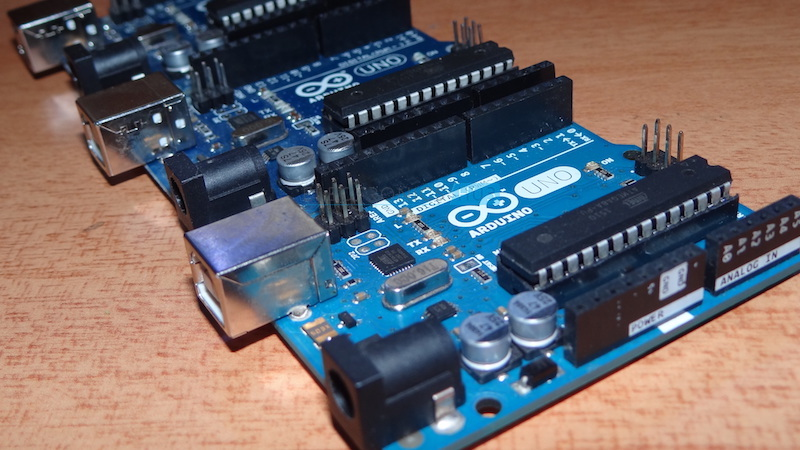
\includegraphics[width=13cm]{1.png}
    \includegraphics[width=13cm]{pic1.png}
    \includegraphics[width=13cm]{pic2.png}
\end{center}

\par\null\par

\textbf{\newline Example 5.6.}\par
$\sigma_{1} = \langle{}a,b\rangle{}$ → $(N, M_0)$
$[\sigma_{1} \rangle{}$ $(N, \lbrack c_2, c_3\rbrack)$\par
$\sigma_{2} = \langle{}a,b,d,e\rangle{}$ → $(N, M_0)$
$[\sigma_{2} \rangle{}$ $(N, \lbrack c_5\rbrack)$\par
$\sigma_{} = \langle{}a,c,d,e,f,b,d,e,g\rangle{}$ → $(N, M_0)$
$[\sigma_{} \rangle{}$ $(N, {\lbrack end}\rbrack)$\par
The set $[N, M_0\rangle{}$ has seven reachable markings.
\par\null\par

\textbf{QUESTION 5.1. On markings in nets, when we have modeled a system as a Petri}\par
\textbf{net system $(N, M_0)$ then some matter occur, including}\par
\begin{enumerate}
    \item How many markings are reachable?
    \item Which markings are reachable?
    \item Are there any reachable terminal markings?
\end{enumerate}
\par
Answer: As we know the initial marking $M_0$ for the given system $(N, M_0)$, we answer such\par questions by calculating the set of markings reachable from $M_0$. We represent this set as a\par
graph - the reachability graph of the net. Its nodes correspond to the reachable\par
markings and its edges to the transitions moving the net from one marking to another.\par 
The key structure is \textbf{reachability graph via transition systems}.
\par\null\par

\begin{center}
    \includegraphics[width=12cm]{Picture24.png}
\end{center}

\textbf{Example 5.7.}\par
Consider the Petri net system in Figure 5.12 modeling the four seasons:\par
\begin{itemize}
    \item Figure 5.12(b) depicts the accompanying reachability graph that represents the set of markings that are reachable from the initial marking shown in figure 5.12(a). We can conclude that the net in figure 5.12(a) has \textbf{four reachable markings}.
    \item The path from marking $[spring]$ to marking $[winter]$ is a finite run $(t1, t2, t3)$ of the net in figure 5.12(a). However, it \textbf{can have infinite run}, as the path can be reduplicated (for example: $(t1, t2, t3, t4, t1, t2, t3), (t1, t2, t3, t4, t1, t2, t3, t4, t1, t2, t3), ...$).
\end{itemize}
\par\null\par

\subsection{Representing Petri Nets as Special Transition Systems}
Let $(N, M_{0})$ with $N = (P,T,F,A,l)$ be a marked labeled Petri net.\par
\begin{center}
    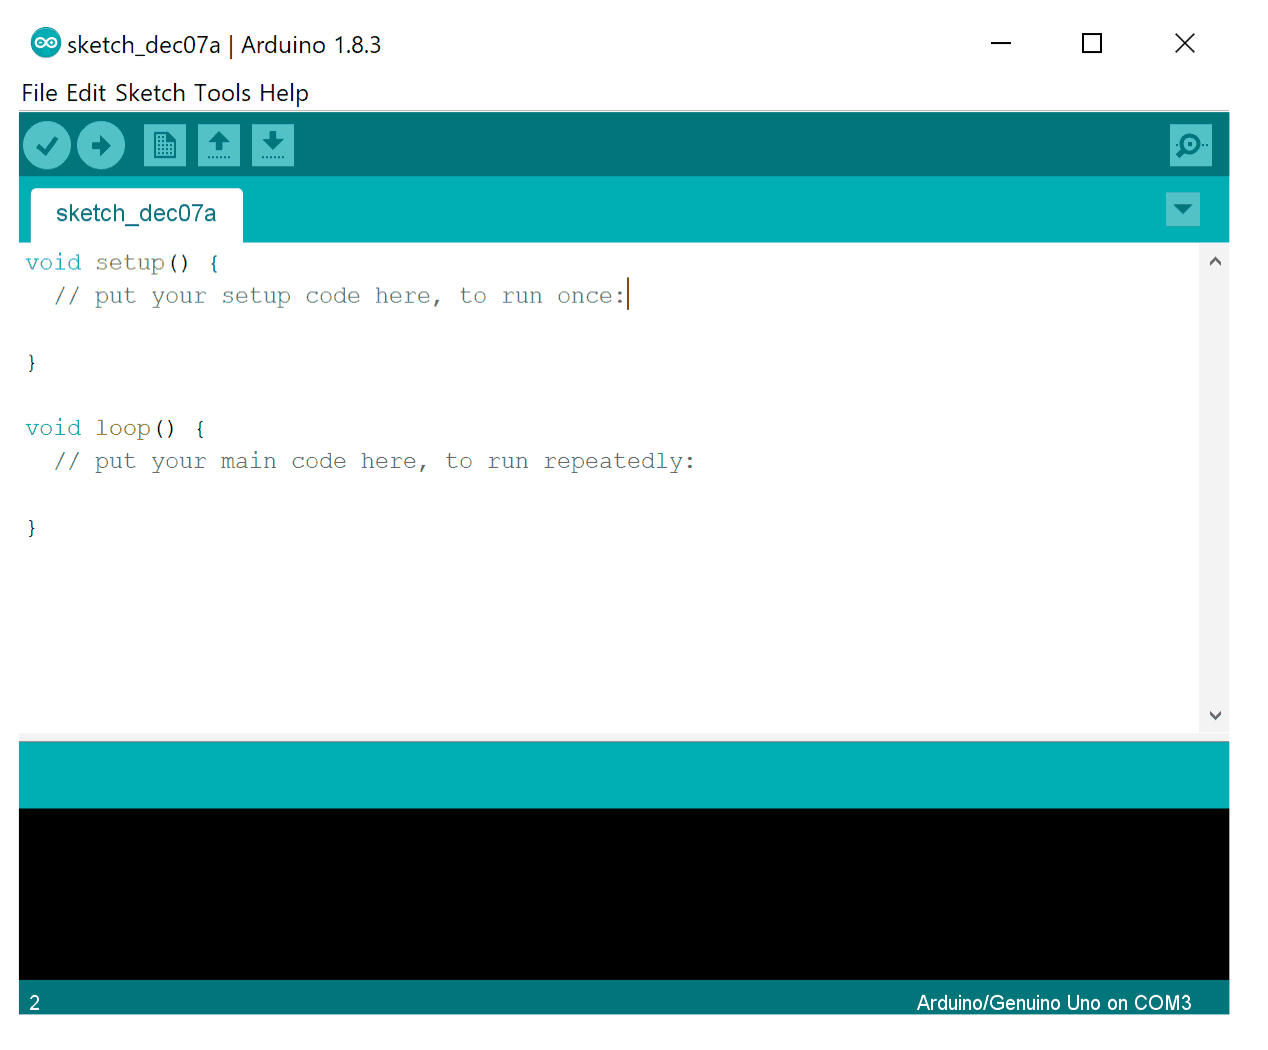
\includegraphics[width=14cm]{2.png}
\end{center}
\textit{After reading ELUCIDATION carefully, we summarize that:}\par
\begin{enumerate}
    \item In this part, the document brings us into the problem of dealing with reachable markings: Sometimes, in the bad situation, we use state transition systems to represent some complex Petri nets in order to categorize places, transitions and avoid forgetting markings.
    \item Moreover, this part provides us some clear materials on how to use the transition systems effectively by the knowledge of multi-set, labeling, sub-graph,...
    \item We also understand more clearly the given examples, thanks to this part as well as some reference books.
\end{enumerate}
\par\null\par
    
\textbf{PRACTICE 5.2.}\par
\begin{center}
    \includegraphics[width=13cm]{Picture25.png}
\end{center}
\par\null\par

\section{PETRI NETWORKS - Structures and Basic Problems}
\textbf{In this part:}
\par\null\par
We know the connecting between token, places and transition. And the document\par
provides materials for us to research the status of token, we try to understand that there are\par
two kind of relationship - Dependence and independence.
\par\null\par
Next, we understand where the token goes and events happen in each cases.\par
In each kinds, there will be a sub-kind, dependence include causality and synchronization.\par
\par\null\par
Moreover, the system that we design must include case in which various events can access or\par
happen at the same time. Next, students need to design the system that allow more threads\par
in order to control the usage of the users and enhance the effective of the system for\par
multiple token.
\par\null\par
For the picture below:
\begin{center}
    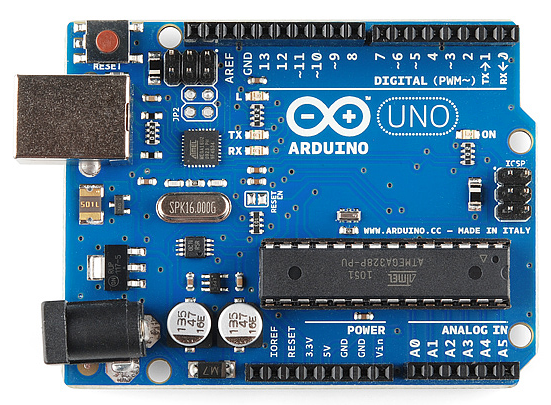
\includegraphics[width=13cm]{4.png}
\end{center}
\par
It helps us to imagine how the Petri net works in 2 different cases: Causality and Concurrency.
\par\null\par
Moreover, the fact that if the model of a process contains a lot of concurrency or multiple\par
tokens reside in the same place, then the transition system TS is much bigger than the Petri\par
net $N = (P, T, F)$.
\par\null\par
Generally, a marked Petri net $(N, M_{0})$ may have infinitely many reachable states.

%%%%%%%%%%%%%%%%%%%%%%%%%%%%%%%%%%%%%%%%%%%%%%%%%%%%%%%%%%%%%%%%%%%%%%%%%%%%%%%%%%%%%%%%%%%%%%%%%%%
\vspace{1 cm}

\section{SUMMARY and REVIEWED PROBLEMS}
\subsection{Problem 5.1}
A Petri net is a particular kind of bipartite directed graphs populated by three types of objects. These objects are places, transitions, and directed arcs. Directed arcs connect places to transitions or transitions to places. In its simplest form, a Petri net can be represented by a transition together with an input place and an output place. This elementary net may be used to represent various aspects of the modeled systems. For example, a transition and its input place and output place can be used to represent a data processing event, its input data and output data, respectively, in a data processing system. In order to study the dynamic behavior of a Petri net modeled system in terms of its states and state changes, each place may potentially hold either none or a positive number of tokens. Tokens are a primitive concept for Petri nets in addition to places and transitions. The presence or absence of a token in a place can indicate whether a condition associated with this place is true or false, for instance.
\par\null\par
1. "enabled transition”: A transition in a Petri net is enabled if each of its input places holds at least one token.\par
e.g: In Figure 5.9, if each of the places $wait$ and $free$ holds at least one token, then\par transition $enter$ is enabled.
\par\null\par
2. "firing of a transition”: An enabled transition can fire, thereby consuming (energy of) one token from each input place and producing at least one token for each output place next.\par
e.g: In Figure 5.10, the enabled transition $enter$ can consume tokens from place $wait$ and\par
$free$ to produce one token to place $before$ and another to place $occupied$.
\par\null\par
3. "reachable marking": A marking $M$ is reachable from the initial marking $M_0$ if and only if there exists a sequence of enabled transitions whose firing leads from $M_0$ to $M$.\par
e.g: In Figure 5.5, the marked Petri net has seven reachable markings.
\par\null\par
4. "terminal marking": The transitions can keep firing until the net reaches a marking that does not enable any transition. Like the terminal state in transition systems, this marking is a terminal marking.\par
e.g: In Figure 5.5, the terminal marking is [end].
\par\null\par
5. "non-deterministic choice": When several transitions are enabled at the same moment, it is not determined which of them will fire. This situation is a non-deterministic choice. Even though we do not know in this case which transition will fire, we know that one of them will be fired.\par
e.g: In Figure 5.5, this situation happens at state $c1$, when there are 2 transitions $b$ and\par
$c$ to fire concurrently or in a certain order.

\subsection{Problem 5.2}
\subsubsection{}
$P = \{p1, p2, p3, p4\}$\newline
$T = \{t1, t2, t3\}$\newline
$F \subseteq (P \times T) \cup (T \times P)$\newline
$M_0 = [1, 0, 1, 2]$
\subsubsection{}
\text{Preset:}
\begin{center}
    \begin{tabular}{|c|c|c|c|c|c|}
    \hline
        $\rightarrow$ & p1 & p2 & p3 & p4\\
    \hline
        t1 & 0 & 1 & 0 & 0\\
    \hline
        t2 & 0 & 0 & 1 & 1\\
    \hline
        t3 & 0 & 0 & 0 & 1\\
    \hline
    \end{tabular}
\end{center}
\text{Postset:}
\begin{center}
    \begin{tabular}{|c|c|c|c|c|c|}
    \hline
        $\leftarrow$ & p1 & p2 & p3 & p4\\
    \hline
        t1 & 1 & 0 & 0 & 1\\
    \hline
        t2 & 0 & 1 & 0 & 0\\
    \hline
        t3 & 0 & 0 & 1 & 1\\
    \hline
    \end{tabular}
\end{center}
\subsubsection{}
At $M_{0}$, transition $t1$ and $t3$ are enabled.
\subsubsection{}
There is no reachable terminal marking.
\begin{center}
    \includegraphics[width=14cm]{Picture26.png}
\end{center}
\subsubsection{}
Non-deterministic choice: $[p4]$
\subsubsection{}
\begin{center}
    \begin{tabular}{c c c c}
        P1 & P2 & P3 & P4\\
        \hline
        1 & 0 & 1 & 2\\
        \hline
        & $\downarrow$ & t1 &\\
        \hline
        0 & 1 & 1 & 1\\
        \hline
        & $\downarrow$ & t2 &\\
        \hline
        0 & 0 & 2 & 2\\
        \hline
        & $\downarrow$ & t3 &\\
        \hline
        0 & 0 & 0 & 2\\
    \end{tabular}
\end{center}
\subsection{Problem 5.3}
\subsubsection{}
$P = \{a,b,c,d,out\}$
$T = \{t1,t2,t3,t4\}$
$M_{0} = \{3,3,3,3,0\}$
\subsubsection{}
Interleaving semantics.\newline
Based on the theory of k-ary n-cube and some widely proven concepts, we have the equation:\newline
The number of vertices: $k^{n}$ vertices\newline
The number of edges:
\begin{itemize}
    \item $nk^{n-1}$ (with k = 2) edges;
    \item $nk^{n}$ (with $k \geq 3$) edges;
\end{itemize}
Therefore, in this problem, as k = 4 and n = 4 (quaternary cube, seen from the graph), we can conclude:
\begin{itemize}
    \item The number of states: 256 ($4^{4}$)
    \item The number of transitions: 1024 ($4 \times 4^{4}$)
\end{itemize}
\subsubsection{}
If we allow concurrency $\Rightarrow$ TS = 15.\newline
$P = \{a,b,c,d,out\}$
\begin{center}
    $\{3, 3, 3, 3, 0\} \xlongrightarrow[\text{TS = 5}]{\text{t1, t2, t3, t4}} \{2, 2, 2, 2, 4\} \xlongrightarrow[\text{TS = 5}]{\text{t1, t2, t3, t4}} \{1, 1, 1, 1, 8\} \xlongrightarrow[\text{TS = 5}]{\text{t1, t2, t3, t4}} \{0, 0, 0, 0, 12\}$
\end{center}

%%%%%%%%%%%%%%%%%%%%%%%%%%%%%%%%%%%%%%%%%%%%%%%%%%%%%%%%%%%%%%%%%%%%%%%%%%%%%%%%%%%%%%%%%%%%%%%%%%%
\vspace{1 cm}

\section{PETRI NETS- ASSIGNMENT on MODELING}

\subsection{Problem 1}
\subsubsection{Write down states and transitions of the Petri net}
Petri net: $N_{S} = (P, T, F)$
\begin{center}
    \includegraphics[width=7cm]{Picture1.png}
\end{center}
$N_{S}$ has three states $P = \{free, busy, docu\}$ and transitions $T = \{start,change,end\}$.
\subsubsection{Represent it as a transition system assuming that}
\subsubsubsection{Each place \textit{cannot} contain more than one token in any marking}
We represent the above Petri net $N_{S}$ as a transition system that a triplet $TS = (S, A, T)$ where $S = \{M_{0}, M_{1}, M_{2}\}$, $A = \{start, change, end\}$, $T = \{T_{1}, T_{2}, T_{3}\}$.\newline
We denote $M_{0}$, $M_{1}$, $M_{2}$ are the marking of Petri net $N_{S}$. Because each state has only one token so there are possibly three markings where $M_{0} = [1, 0, 0]$, $M_{1} = [0, 1, 0]$, $M_{2} = [0, 0, 1]$. Because state \textit{free} are both initial and final states since then $M_{0}$ is also both initial and final states. Then \textit{T} is set of transition where $T_{1}\{M_{0}, free, M_{1}\}$, $T_{2}\{M_{1}, change, M_{2}\}$, $T_{3}\{M_{2}, end, M_{0}\}$.
\begin{center}
    \includegraphics[width=12cm]{Picture2.png}
\end{center}
\subsubsubsection{Each place may contain any natural number of tokens in any marking}
We can formalize the states as $S = \{(x,y,z) | x,y,z \in N\}$. The initial state $s_0$ is equal to the initial marking $m_0 = (1,0,0)$. The transition relation can be specified by the union of the following three sets:\newline
$ TR = \{((x+1,y,z),(x,y+1,z)) | x,y,z \in N\}$\par
$\cup \{((x,y+1,z),(x,y,z+1)) | x,y,z \in N\}$\par
$\cup \{((x,y,z+1),(x+1,y,z)) | x,y,z \in N\}$\newline
the first, the second, and the third set contains all possible states that can be reached by firing transition start, change, and end, respectively.

\subsection{Problem 2}
We define Petri net $N_{Pa} = (P, T, F)$ where $P = \{wait, inside, done\}$, $T = \{start, change\}$.
\subsubsection{Explain the possible meaning of a token in state inside of the net}
We define a token in state $inside$ as a patient being treated by the specialist. In other words, we evaluate the state $inside$ similar to the state $busy$ of the $N_s$ Petri net model.
\subsubsection{Construct the Petri net, assuming that there are five patients in state wait, no patient in state inside, and one patient is in state done}
The tokens in place $wait$ represent the waiting patients. Transition $start$ and $change$ represent two possible events. the transition $start$ firing that transfer tokens from state $wait$ into state $inside$ and then transition $change$ firing that transfer tokens from states $inside$ into states $done$. 
\begin{center}
    \includegraphics[width=\textwidth]{Picture4.png}
\end{center}

\subsection{Problem 3}
We construct $N = N_{S} \oplus N_{Pa} = (P, T, F)$, and $P_{N} = P_{S} \cup P_{Pa}$, $T_{N} = T_{S} \cup T_{Pa}$, $F_{N} = F_{S} \cup F_{Pa}$.\newline
Since we define $busy$ and $inside$ as the concurrency states so
\begin{center}
    $P_{N} = \{free, wait, (busy|inside), docu, done\}$
\end{center}
and
\begin{center}
    $T_{N} = \{start, change, end\}$
\end{center}
Then we can have the model below:
\begin{center}
    \includegraphics[width=\textwidth]{Picture5.png}
\end{center}

\subsection{Problem 4}
The reachable markings from $M_0$ by firing one transition once are:
\begin{center}
    $M_{0} \rightarrow M_{1}[2.wait, (busy|inside), done] \rightarrow M_{2}[2.wait, docu, 2.done] \rightarrow M_{3}[2.wait, free, 2.done] \rightarrow M_{4}[wait, (busy|inside), 2.done] \rightarrow M_{5}[wait, docu, 3.done] \rightarrow M_{6}[wait, free, 3.done] \rightarrow M_{7}[(busy|inside), 3.done] \rightarrow M_{8}[docu, 4.done] \rightarrow M_{9}[free, 4.done]$
\end{center}

\subsection{Problem 5}
The Petri net N is not deadlock free because there exists a terminal marking which no longer enables any transition. For example, if we construct an initial marking $M_0$ $[1.free,5.done]$ so this initial making is deadlock and then Petri net N is not deadlock free.
\begin{center}
    \includegraphics[width=\textwidth]{Picture6.png}
\end{center}

\subsection{Problem 6}
We have 2 ideas about Petri net model for 2 specialists.\newline
First Petri net we define 2 kinds of tokens in one state free that representing 2 specialists.
\begin{center}
    $N_{1} = (P, T, F)$
\end{center}
where
\begin{center}
    $P = \{free, wait, inside, docu, done\}$,
    $T = \{start, change, end\}$
\end{center}
The tokens in state \textit{free} represent the specialist is free and waits for the next patient. The tokens in state \textit{wait} represent the patient is waiting, one in state \textit{inside} represent the specialist is busy treating the doctor is treating as well as the patient being treated by the doctor. And then state \textit{docu} represent the specialist is documenting the result of the treatment and the end \textit{done} states represent the patient has been treated by the specialist.
\newline
Then construction $N_{1}$ below the initial marking $M_{0} = [2.free, 5.wait]$:
\begin{center}
    \includegraphics[width=\textwidth]{Picture7.png}
\end{center}
The second idea 
\begin{center}
    $N_{2} = (P, T, F)$
\end{center}
where
\begin{center}
    $P = \{free1,free2,wait,inside1,inside2,docu1,docu2,done\}$,
    $T = \{start1,start2,change1,change2,end1,end2\}$
\end{center}
With the tokens in states \textit{free1} and \textit{free2} represent the \textit{specialist1} and \textit{specialist2} are free respectively and waits for the next patient. The tokens in state \textit{wait} represent the patient is waiting, one in state \textit{inside1} and \textit{inside2} represent the \textit{specialist1} and \textit{specialist2} are busy treating the doctor is treating as well as the patient being treated by the doctor respectively. And then state \textit{docu1} and \textit{docu2} represent the \textit{specialist1} and \textit{specialist2} are documenting the result of the treatment respectively and the end \textit{done} states represent the patient has been treated by the specialist.
\newline
The construction $N_{2}$ below with initial marking $M_{0}[free1, free2, 3.wait]$:
\begin{center}
    \includegraphics[width=\textwidth]{Picture8.png}
\end{center}
The tokens inside states \textit{free}, \textit{free1}, \textit{free2} is no more than one token. State \textit{wait}, gets value \textit{n} if there are \textit{n} patients waiting.

\subsection {Problem 7}
\subsubsection{[Package description]}
Language used: R
\par\null\par
[ITEM 1] PATIENT NETWORK\par
This program allows:\par
1) MAX: 10 patients in place wait.\par
2) Only one patient being treated at a time.\par
3) The process will run until there is no patient left in the waiting room.
\par\null\par
[ITEM 2] SPECIALIST NETWORK\par
This program allows: \par
1) MAX: 1 specialist on duty.\par
2) Only one patient being treated at a time.\par
3) The number of firing times will define the final display.
\par\null\par
[ITEM 3] SUPERIMPOSED NETWORK\par
This program allows: \par
1) MAX: 10 patients in place wait and 1 specialist on duty.\par
2) Only one patient being treated at a time.\par
3) The process will run until there is no patient left in the waiting room.
\par\null\par
[ITEM 4] CALCULATOR
\subsubsection{[Source code]:}
\href{https://drive.google.com/drive/folders/1G4_9ujAwx-T7atTZgRQO23wBjPQ4VADA?usp=sharing}{Click here}


\vspace{2 cm}

\begin{thebibliography}{80}


\bibitem{bib1}
\url{https://en.wikipedia.org/wiki/Petri_net}

\bibitem{bib2}
\url{https://www.sciencedirect.com/topics/physics-and-astronomy/petri-nets}

\bibitem{bib3}
\url{http://www.scholarpedia.org/article/Petri_net}

\bibitem{bib4}
Girault C, Valk R (2003) Petri Nets for systems engineering. Springer, New York

\bibitem{bib5}
Peterson JL (1981) Petri Net theory and the modeling of systems. Prentice-Hall, Englewood Cliffs

\bibitem{bib6}
Murata T (Apr 1989) Petri nets: properties, analysis and applications. Proc IEEE 77(4):541–580

\bibitem{bib7}
Modeling business processes a Petri net-oriented approach by Aalst, Wil van der Stahl, Christian

\bibitem{bib8}
PROCESS MINING, 2nd edition, 2016, Springer, by W.M.P.Aalst, van der

\bibitem{bib9}
DATA MINING- Concepts, Models, Methods, and Algorithms,
3rd Edition, 2020, IEEE press and Wiley, by Mehmed Kantardzic

\end{thebibliography}
\end{document}

